\documentclass[]{beamer}
% \geometry{papersize={16cm,9.60cm}}
\usepackage{etex}
\usepackage{amsmath}
\usepackage{tikz}
\usepackage{multimedia}
\usetheme{Boadilla}
\usepackage{graphicx}
%\usepackage{inputenc}

% \mode<presentation>
% {
%   \usetheme{default}
%   \setbeamercovered{transparent}
% }


% {\vskip5pt}

%% customize layout, bullet points navigation toolbar
\setbeamertemplate{navigation symbols}{}%remove navigation symbols
\setbeamertemplate{enumerate items}[default]
\setbeamertemplate{navigation symbols}{}
\setbeamertemplate{itemize items}[circle]
\setbeamercolor{enumerate item}{fg=black}

\setbeamertemplate{footline}{}
\setbeamersize{text margin left = 2.0em}
\setbeamersize{text margin right = 2.0em}

\usepackage{times}
\usepackage[T1]{fontenc}

% Or whatever. Note that the encoding and the font should match. If T1
% does not look nice, try deleting the line with the fontenc.

\setbeamertemplate{navigation symbols}{}

\title{ Cognitive (Neuro) Psychology }
\subtitle{I. Introduction}
\author{ Marianne Maertens }
\institute[TU Berlin]{Technische Universit\"at Berlin}
\date{July 2016}

\begin{document}
\setbeamertemplate{enumerate items}[default]
\setbeamertemplate{headline}

\frame{\titlepage}

\AtBeginSection[]
{
  \begin{frame}<beamer>
    \frametitle{Layout}
    \tableofcontents[currentsection]
  \end{frame}
}


\begin{frame}
 \frametitle{Your lecturer}
\begin{columns}[T]
 \begin{column}{80mm}
\begin{itemize}
 \item[]<1-> \textbf{background:} psychology
 \item[]<2-> \textbf{research interest:} visual perception: experiments \& models
 \item[]<4-> \textbf{location:} TU Berlin
 \item[]<5-> \textbf{group:} Christiane, Guillermo, Torsten 
\end{itemize}
  \end{column}

\begin{column}{40mm}
\includegraphics<2>[width=30mm]{../../../figures/anderson_chess.jpg} 
% \includegraphics<2>[width=30mm]{../../../figures/varin_thin.png} 
\includegraphics<4>[width=30mm]{../../../figures/marchstrasse_building.jpg} 
\includegraphics<3>[width=40mm]{../../../figures/odog_model.png}
\end{column}
\end{columns}
\end{frame}


\begin{frame}
 \frametitle{So far ...}

\begin{itemize}
\setlength{\itemsep}{5pt}
 \item Introduction to Neurobiology
 \item Sensory Physiology
 \item Programming
 \item<2-> \textcolor{blue}{Cognitive (Neuro)Psychology}
\end{itemize}
\end{frame}

\begin{frame}
 \frametitle{What do you expect?}
\end{frame}


\begin{frame}
 \frametitle{Objectives}
 basic knowledge in
\begin{itemize}
  \item Cognitive Psychology
  \item Neuropsychology
  \item Experimental Methods
\end{itemize}

\only<2->{
\begin{itemize}
 \item What kind of questions are addressed in the discipline?
 \item How are these questions being addressed?
 \item Be able to comprehend and evaluate literature and work done in the field.
\end{itemize}
}
\end{frame}

\begin{frame}
 \frametitle{Topics \& Structure}
\begin{center}
\includegraphics<1>[width=100mm]{figs/l1/block_I.png} 
\includegraphics<2>[width=100mm]{figs/l1/block_II.png} 
\end{center}
\end{frame}

\begin{frame}
 \frametitle{Philosophy}
\begin{overlayarea}{110mm}{50mm}
Challenge: block course!! \\
\vspace{5mm}
\only<2->{
 \begin{itemize}
  \item alternation between instruction and individual studies
  \item active involvement of participants
  \item some topics in depth instead of broad coverage
  \item exam: indicate the degree of retention of material - MC 
  \item[]
  \item<3->[!] What do I expect?
 \end{itemize}
}
\end{overlayarea}
\end{frame}


\begin{frame}
 \frametitle{Outline for today}
\begin{itemize}
 \item Demarcation
 \item Approaches to Cognition
\end{itemize}

\end{frame}


\begin{frame}
 \frametitle{Human cognition}
\begin{columns}[T]
 \begin{column}{60mm}
 Internal processes involved in making sense of the environment and deciding what action might be appropriate. \\
\begin{itemize} 
 \item attention
 \item perception
 \item learning
 \item memory
 \item language
 \item problem solving
 \item reasoning
 \item thinking
\end{itemize}
 \end{column}
\begin{column}{50mm}
\includegraphics<1>[width=50mm]{figs/the_mind_SebastianEriksson.jpg} 
\end{column}
\end{columns}
\end{frame}




\begin{frame}
\frametitle{Human cognition}
 \begin{center}
\includegraphics<1>[width=110mm]{../../../figures/adelson_processing.png}
 \end{center}
\end{frame}


\begin{frame}
 \begin{exampleblock}{Thinking}
You cannot observe atoms directly. We still think they
exist. Why? We cannot observe thoughts in other people
directly. We still think they exist. Why?
 \end{exampleblock}
\end{frame}


\begin{frame}
 \frametitle{Approaches to Human Cognition}
 \begin{enumerate}
  \item Cognitive Psychology
  \item Cognitive Neuropsychology
  \item Cognitive Neuroscience
  \item Computational Cognitive Science 
 \end{enumerate}
\end{frame}


\begin{frame}
\frametitle{What is Cognitive Psychology?}
Scientific attempt to understand human cognition by observing the behavior of people performing various cognitive tasks.
\end{frame}


\begin{frame}
\frametitle{What is Cognitive Psychology?}

 \begin{columns}[T]
 \begin{column}{70mm}
\begin{overlayarea}{70mm}{70mm}
  \begin{itemize}
   \item Miller (1956) - magical number 7$\pm$2
   \item Bruner, Goodnow, \& Austin (1956) - a study of thinking 
   \item \textcolor<2->{blue}{Broadbent (1958) - filter theory}
   \item Newell \& Simon (1972) - a general problem solver
   \item ...
   \item[]
   \item<3->[$\Rightarrow$] capacity limits
  \end{itemize}
\end{overlayarea}
 \end{column}
  
 \begin{column}{40mm}
\begin{center}
 \includegraphics<2->[width=35mm]{../../../figures/dichotic_listening_task.png}
\end{center}
 \end{column}
 \end{columns}
\end{frame}


\begin{frame}
 \frametitle{The computer metaphor}
\begin{center}
Cognition as information processing approach\\
\vspace{5mm}
bottom-up $\longleftrightarrow$ top-down processing
\end{center}

\begin{exampleblock}{Thinking}
  In what way is your brain like a digital computer? What
are the differences? Do they matter for the computer
metaphor?
\end{exampleblock}

\only<2>{
\begin{itemize}
 \item Cognitive Science - Cognitive Systems - Artificial Intelligence 
\end{itemize}
}
\end{frame}



\begin{frame}
\frametitle{Human cognition}
 \begin{center}
\includegraphics<1>[width=110mm]{../../../figures/adelson_brain_processing.png}
 \end{center}
\end{frame}

\begin{frame}
 \frametitle{Cognitive Neuropsychology}
\begin{overlayarea}{110mm}{70mm}
 \begin{itemize}
 \setlength{\itemsep}{5pt}
 \item[Idea:] look at patterns of cognitive performance (intact and impaired) shown by brain-damaged patients
 \item[!] the principle aim is not to learn about the brain, but to elucidate the functional architecture of cognition
\end{itemize}

\only<2->{
\textcolor{blue}{Assumptions:}
\begin{itemize}
 \item Modular organization: functional \& anatomical
 \item Subtractivity: brain damage impairs modules does not add them
\end{itemize}
}
\end{overlayarea}

\end{frame}


\begin{frame}
\frametitle{Double dissociation}
 \begin{center}
\includegraphics<1>[width=110mm]{../../../figures/mishkin_double_diss.png}

\begin{footnotesize}Mishkin, 1983\end{footnotesize}
 \end{center}

\begin{itemize}
 \item[A] lesions in ventral stream impair object identification, but not localization
 \item[B] lesions in dorsal stream impair object localization, but not identification
\end{itemize}
\end{frame}

\begin{frame}
\frametitle{Dissociation}
 \begin{center}
\includegraphics<1>[width=50mm]{../../../figures/ebbinghaus.png}
\includegraphics<1>[width=50mm]{../../../figures/ebbinghaus_grasping.png}

\includegraphics<2>[width=100mm]{../../../figures/goodale_nature91_results.png}

\only<2->{\begin{footnotesize}Goodale et al., 1991\end{footnotesize}}
 \end{center}
\only<1>{
\begin{itemize}
 \item damage ventrally in lateral occipital region
\end{itemize}
}
\end{frame}

\begin{frame}
\frametitle{Cognitive Neuropsychology - A critical evaluation}
\begin{itemize}
 \item different patients have different and diffuse lesions 
 \item patients often impaired in more than one function, secondary effects
 \item interruption of a function by a lesion does not mean that
the function is localized in the respective area
 \item strongest evidence comes from double dissociations but is
not fool-proof
 \item functions may still be distributed over the brain and not
localized in one area - why?
\end{itemize}
\end{frame}

\begin{frame}
 \frametitle{Cognitive Neuroscience}

\begin{itemize}
 \item 1928 - 1947 Penfield stimulated brains during brain surgery
 \item[] "those fingers and my thumb gave a jump" - stimulation near central sulcus
 \item[]
 \item[$\Rightarrow$] How are mental processes such as thoughts, memories and perceptions organized and implemented by the brain?
\end{itemize}
\end{frame}


\begin{frame}
\frametitle{Cognitive Neuroscience}
 \includegraphics<1>[width=110mm]{figs/methods_overview.png}
% \includegraphics<2>[width=110mm]{figs/methods_classification.png}
\end{frame}



\begin{frame}
 \frametitle{Single cell / multi-unit recording}
\begin{center}
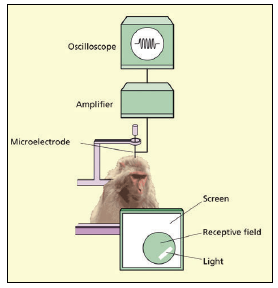
\includegraphics[width=60mm]{figs/l3/ward_single_cell_recording.png} 
\end{center}
\end{frame}

\begin{frame}
 \frametitle{EEG}
\begin{center}
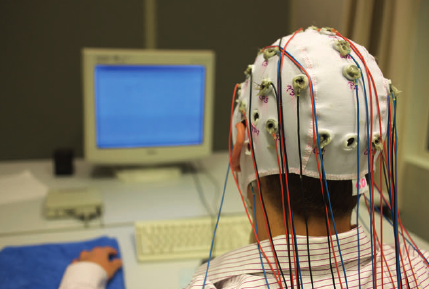
\includegraphics[width=50mm]{figs/l1/eeg_cap.png} 

\vspace{3mm}
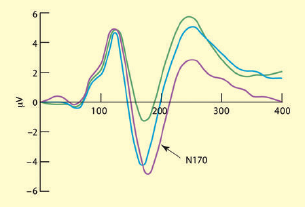
\includegraphics[width=50mm]{figs/l1/erp_face_animal_object.png} 
\end{center}
\end{frame}

\begin{frame}
 \frametitle{fMRI}
\begin{center}
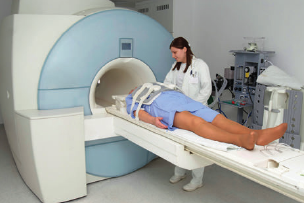
\includegraphics[width=45mm]{figs/l1/fmri_magnet.png} 

\vspace{3mm}
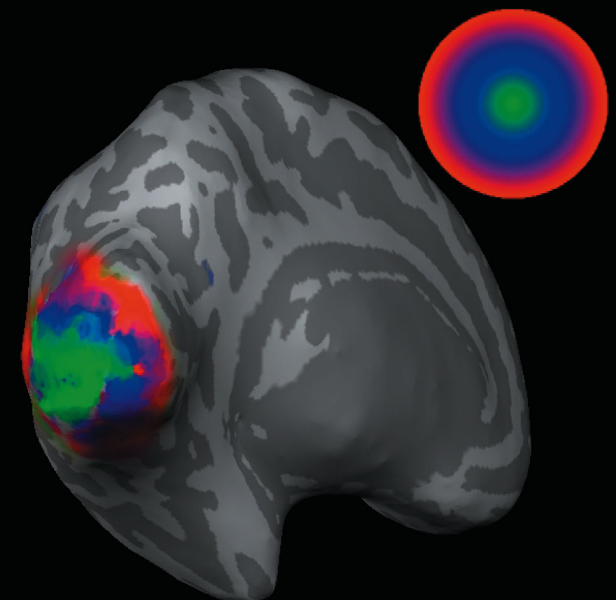
\includegraphics[width=45mm]{figs/l1/fmri_flat_map.png} 
\end{center}
\end{frame}

\begin{frame}
 \frametitle{TMS}
\begin{center}
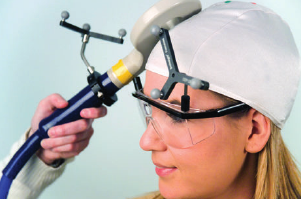
\includegraphics[width=55mm]{figs/l1/tms.png} 
\end{center}
\end{frame}


\begin{frame}
\frametitle{Cognitive Neuroscience}
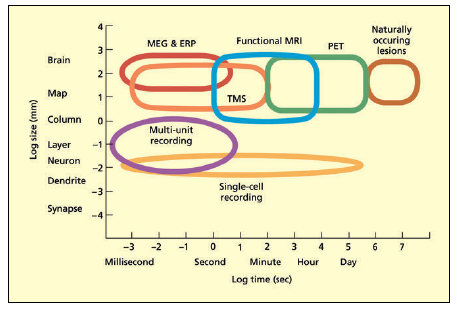
\includegraphics[width=110mm]{figs/methods_classification.png}
\end{frame}

\begin{frame}
\frametitle{fMRI - decoding}
 \includegraphics<1>[width=110mm]{../../../figures/haxby_science01.png}
\end{frame}


\begin{frame}
\frametitle{Cognitive Neuroscience - a critical evaluation}

\begin{columns}[T]
 \begin{column}{70mm}
\begin{overlayarea}{70mm}{70mm}
\begin{itemize}
\setlength{\itemsep}{10pt}
 \item blobology - activation in a small area is interpeted as the 'love' area
 \item reverse inference - infer involvement of a cognitive process based on activation within a given brain area
 \item 'neuroimaging illusion' 
\end{itemize}
\end{overlayarea}
 \end{column}

 \begin{column}{50mm}
\begin{center}
\includegraphics<2>[width=50mm]{../../../figures/keehner_psych11_results.png}

\only<2->{\begin{footnotesize}Keehner et al., 2011\end{footnotesize}}
 \end{center}
 \end{column}
\end{columns}
\end{frame}




\begin{frame}
 \frametitle{Computational Cognitive Psychology}
 \begin{itemize}
  \item program computers to mimic aspects of human cognitive functioning
  \item [!AI] construct systems that produce intelligent behavior but bear little resemblance to those used by humans e.g. deep blue
 \item a good computational model shows us how a given theory can be specified and allows us to predict behavior in new situations
 \item  requires the researcher to be explicit about a theory in a way a verbal theory does not
 \item specific $\longleftrightarrow$ generic 
 \end{itemize}
\end{frame}



\begin{frame}
\begin{overlayarea}{120mm}{70mm}
\begin{center}
  What does it mean to understand something, e.g. perception? 
\end{center}

\only<2->{
\begin{center}
\begin{itemize}
\centering
 \item[] Neurophysiology 
 \item[] Psychology 
 \item[] Computational Neuroscience
 \item[] Neuropsychology
 \item[] Pharmacology
 \item[] Robotics
 \item[] ...
\end{itemize}
\end{center}
}

\end{overlayarea}
\end{frame}


\begin{frame}
  \begin{center}  
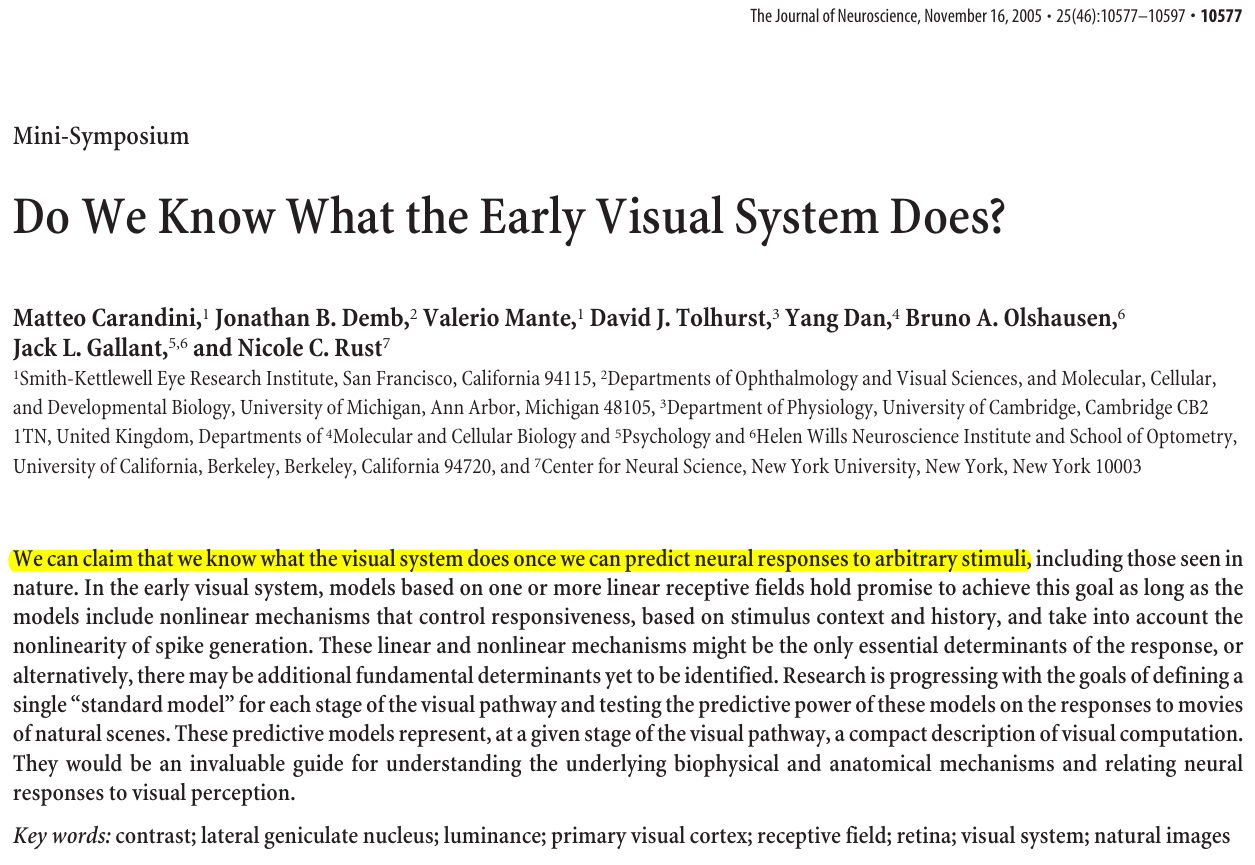
\includegraphics[width=110mm]{figs/what_early_visual_system.png}
  \end{center}
\end{frame}



\begin{frame}{What does it mean to understand something?}

\begin{overlayarea}{110mm}{75mm}
\begin{columns}[T]
\begin{column}{40mm}
\vspace{6mm}
\begin{center}  
\textbf{C. elegans} 
\end{center}
\end{column}
\begin{column}{60mm}
  \begin{center}  
\includegraphics[width=50mm]{../../../figures/c_elegans.jpg}
  \end{center}
\end{column} 
\end{columns}


\begin{itemize}
 \item<2-> complex behavior - chemotaxis, thermotaxis and thermo memory ...
 \item<3-> complete knowledge of the components of its biological hardware 
\begin{itemize}
 \item<3-> 302 nerve cells, 'wiring diagram' completed
 \item<3->  600 gap junctions, 5000 chemical synapses, neurotransmitters and neuromodulators known 
 \item<3->  19099 genes completely sequenced
\end{itemize}
\item<4> ``Surprisingly little progress has been made in understanding these (behavioral) responses''
\end{itemize}
\end{overlayarea}
\begin{center}
\only<4->{\scriptsize{[after Mausfeld, 2003]}}
\end{center}
\end{frame}



\begin{frame}{What does it mean to understand something?}

\begin{overlayarea}{110mm}{70mm}
\begin{columns}[T]
\begin{column}{60mm}
\vspace{5mm}
\begin{center}
  What does it mean to have understood visual perception?
\end{center}
\end{column}
\begin{column}{50mm}
  \begin{center}  
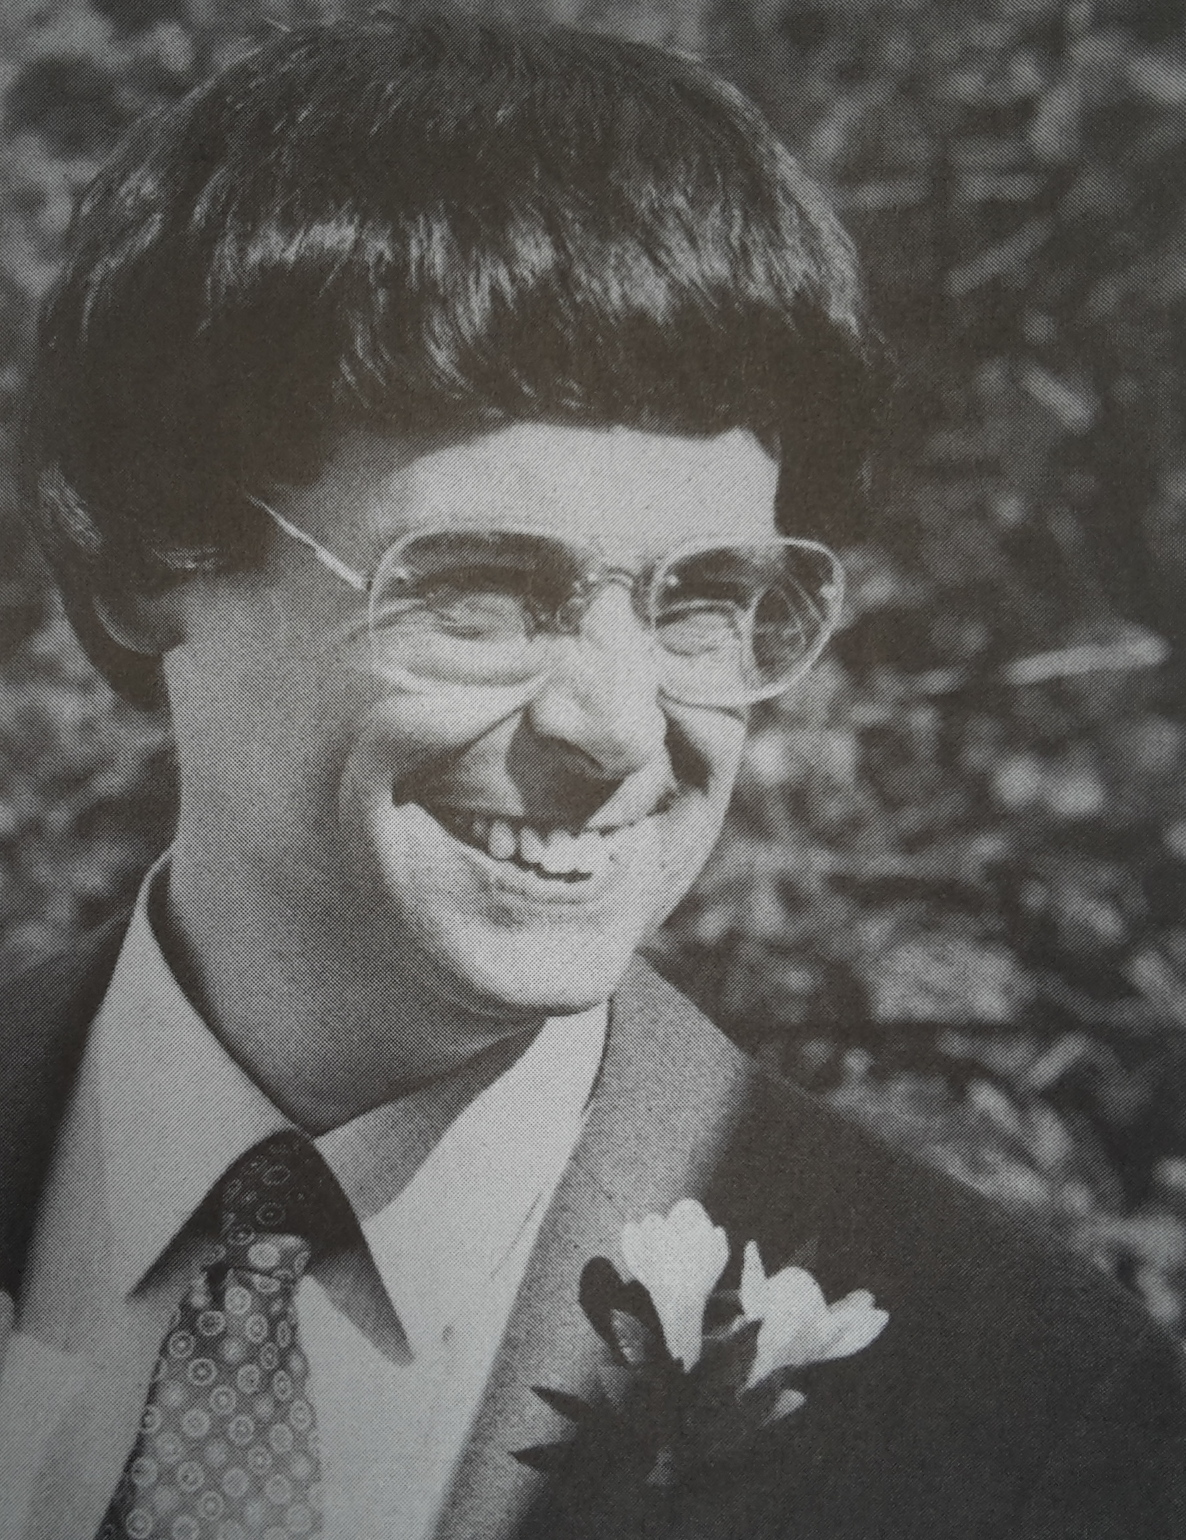
\includegraphics[width=30mm]{figs/marr.jpg}
  \end{center}
\end{column}
\end{columns}

\only<2->{
\begin{itemize}
 \item visual perception as an information processing system
 \item complex systems should be understood at several different levels 
 \item use every bit of information, every approach, every technique that is available to us
\end{itemize}
}
\end{overlayarea}
\begin{center}
\scriptsize{[Marr, 1982, 2010]}
\end{center}
\end{frame}



\begin{frame}
\frametitle{What is the problem in vision?}
\begin{columns}[T]
 \begin{column}{50mm}
  \begin{center}  
   \includegraphics<1-2>[width=33mm]{../../../figures/dress.jpg}
  \end{center}
\tiny{
\url{
http://swiked.tumblr.com/post/112073818575/guys-please-help-me-is-this-dress-whi
te-and}}
 \end{column}
 \begin{column}{60mm}
  \only<2->{
  \begin{center}  
   \includegraphics[width=58mm]{../../../figures/dress_brainard.png}
  \end{center}

\begin{center}
\tiny{Hurlbert \& Brainard, 2015; Gegenfurtner et al., 2015}
\end{center}
}
 \end{column}
\end{columns}
\end{frame}


\begin{frame}{The retinal input is ambiguous}
\begin{center}
\includegraphics<1>[width=70mm]{../../../figures/adelson_demo_bar.png}

\tiny{\only<1>{[after Adelson, 1995]}}
\end{center}
\end{frame}


\begin{frame}{How does the visual system resolve sensory ambiguity?}
\begin{overlayarea}{110mm}{65mm}
\begin{center}
\includegraphics[width=110mm]{../../../figures/adelson_image_processing.png}
\end{center}

\only<2>{
\begin{columns}[T]
\begin{column}{30mm}
\begin{itemize}
 \item computation
\end{itemize}
\end{column}

\begin{column}{70mm}
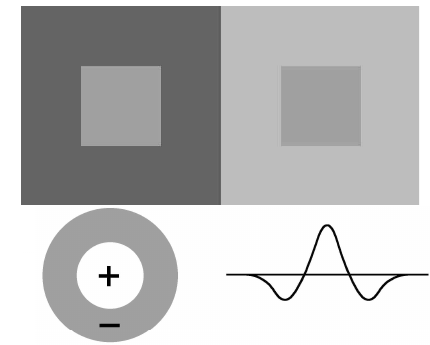
\includegraphics[width=35mm]{figs/adelson_SBC_center_surround.png}

\scriptsize{[Adelson, 2000]}
\end{column}
\end{columns}
}

\only<3->{
\vspace{5mm}
\begin{itemize}
 \item [$\Rightarrow$] \textcolor{blue}{computational goal} 
%  \item color is the perceptual approximation to reflectance
%  \item[] \textit{How can the effects of reflectance changes be separated from the vagaries of the prevailing illumination?} 
%  \item[] \scriptsize{[p. 17, Marr, 2010]}
\end{itemize}
}
\end{overlayarea}
\end{frame}



\begin{frame}{Computational goal}
\begin{overlayarea}{110mm}{50mm}
\begin{columns}[T]
\begin{column}{27mm}
\vspace{5mm}
$I(x,y)$
\begin{itemize}
 \item \textcolor<3>{blue}{geometry}
 \item \textcolor<3>{blue}{reflectance}
 \item[]
 \item illumination
 \item viewpoint
\end{itemize}

\end{column}
\begin{column}{83mm}
  \begin{center}  
\includegraphics[width=83mm]{../../../figures/marr_intensity_adelson.png}
  \end{center}
\end{column}
\end{columns}
\end{overlayarea}

\begin{itemize}
  \item<2->[$\Rightarrow$] sort out which changes are due to what factors
  \item<3->[$\Rightarrow$] create representations in which coincidental fluctuations are separated from changes that are diagnostic for \textcolor<3>{blue}{\textbf{invariant}} object properties
\end{itemize}
\end{frame}


\begin{frame}
 \frametitle{Marr's three levels}
\begin{overlayarea}{100mm}{55mm}
\begin{small}
 \begin{tabular}{ll}
\hline
 \textit{\begin{tabular}[l]{@{}l@{}} Computational \\ theory\end{tabular}} & \begin{tabular}[l]{@{}l@{}} What is the goal of the computation, \\ why is it appropriate, and what is the logic \\ of the strategy by which it can be carried out? \end{tabular} \\
\hline


\textit{ \begin{tabular}[l]{@{}l@{}} Representation \\and algorithm \end{tabular}} &  \begin{tabular}[l]{@{}l@{}} How can this computational theory be implemented? \\ In particular, what is the representation for  the \\ input and output, and what is the algorithm \\for the transformation?  \end{tabular} \\ \hline

\textit{\begin{tabular}[l]{@{}l@{}} Hardware \\ Implementation \end{tabular}} & \begin{tabular}[l]{@{}l@{}}How can the representation and algorithm be \\ realized physically? \end{tabular} \\ \hline 
 \end{tabular}
\end{small}
\end{overlayarea}

\begin{itemize}
 \item<2>[$\rightarrow$]\textcolor{blue}{Understanding perception requires answers at all levels}
\end{itemize}

\begin{center}
\scriptsize{[Marr, 1982, 2010]}
\end{center}
\end{frame}

 
\begin{frame}
 ``We cannot develop a rigorous theory of early vision unless we know what the theory is for [Marr, 2010, p.41]. ''\\
\vspace{5mm}
\only<2-> {``[...] trying to understand perception by studying only neurons is like trying to understand bird flight by studying only feathers: It just cannot be done. In order to understand bird flight, we have to understand
aerodynamics; only then do the structure of feathers and the different shapes of birds' wings make sense.'' [Marr, 2010, p. 27]}
\end{frame}




\begin{frame}{Example}
 \begin{overlayarea}{110mm}{35mm}
\begin{columns}[T]
 \begin{column}{30mm}
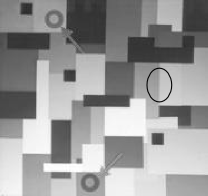
\includegraphics[width=30mm]{figs/mondrian_edge.png}
 \end{column}

 \begin{column}{80mm}
\includegraphics<3->[width=80mm]{figs/luminance_zero.jpg}
 \end{column}
\end{columns}
\end{overlayarea}
\textcolor{blue}{computational goal:}
\begin{itemize}
 \item  separate illumination from reflectance changes 
 \item<2->[$\rightarrow$] separate gradual from sharp intensity changes
\item[]
 \item<3-> intensity steps in an image (a) are peaks in the first derivative (b) across the steps, or zero-crossings in the second derivative (c)
 \item<4-> intensity steps can efficiently be detected with a differential operator 
\end{itemize}
\end{frame}


\begin{frame}{Example}
 \begin{center}
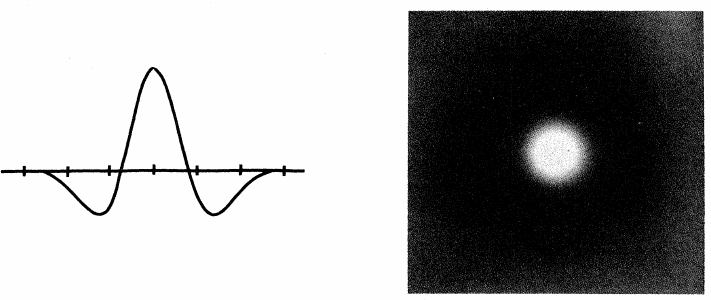
\includegraphics[width=60mm]{figs/marr_hildred_mexican_hat.png}
\end{center}
 \begin{itemize}
 \item the second derivative can be found by filtering the image with a Mexican hat function (Marr-Hildreth algorithm )  
\item[=] \textcolor{blue}{algorithmic level}
  
 \item<2-> resemblance to concentric center-surround organization of neurons in the LGN
 \item<2->[=] \textcolor{blue}{implementational level} 
\end{itemize}
\end{frame}


\begin{frame}{From images to the primal sketch}
 \begin{center}
\includegraphics<1>[width=60mm]{figs/marr_primal_sketch.png}
\end{center}
 \end{frame}



\begin{frame}{From images to 3D-objects}
 \begin{center}
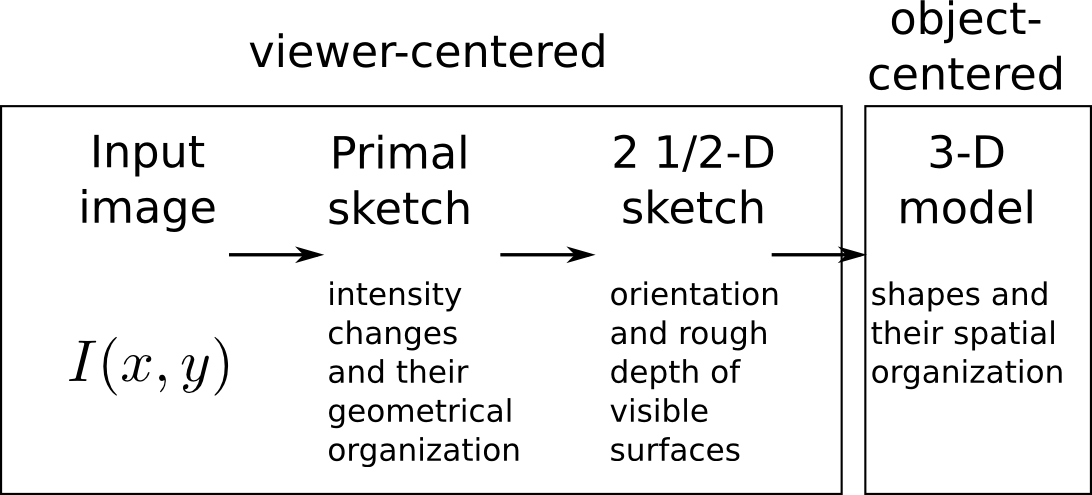
\includegraphics[width=100mm]{figs/marr_representations.png}
\end{center}
\end{frame}



\begin{frame}
 \frametitle{Summary}
\begin{itemize}
\setlength{\itemsep}{5pt}
 \item Cognitive Psychology is the experimental study of human cognition
 \item Cognitive Psychology combines a number of different approaches including behavioral experiments, computational modelling and the study of the brain
 \item Cognitive Psychology focusses on the study of human cognition and as such is a subfield of Cognitive Science which also considers other cognitive agents
 \item The study of Human Cognition becomes increasingly transdisciplinary recognizing the\textbf{ usefulness of a diverse set of different approaches}
\end{itemize}
\end{frame}


% 
% \begin{frame}
% \frametitle{Tutorial: how to measure perception?}
% \begin{center}
% \includegraphics<1>[width=60mm]{../../../figures/bregman_Bs.png}
% \includegraphics<2>[width=20mm]{../../../figures/banana_penetrates_brick.png}
% \includegraphics<3>[width=60mm]{../../../figures/amodal_michotte.png}
% \end{center}
% \end{frame}
% 
% \begin{frame}
%  \begin{exampleblock}{Thinking}
%  How can you find out what's happening in someone's
% head? In normal life? In science?
%  \end{exampleblock}
% \end{frame}
% 


\begin{frame}
 \frametitle{References}
\begin{small}
\begin{itemize}
 \item  Eysenck \& Keane (2010). Cognitive Psychology. A student's handbook. 
 \item Ward, J. (2010). The student's guide to cognitive neuroscience (2nd ed.). Taylor \& Francis, Psychology Press: Hove and New York.
 \item Marr, D. (2010). Vision.  
\end{itemize}
\end{small}
\end{frame}


\end{document}